\documentclass[11pt,a4paper]{article}

\usepackage[utf8]{inputenc}
\usepackage[T1]{fontenc}
\usepackage[spanish]{babel}
\usepackage{lmodern}
\usepackage{microtype}
\usepackage[margin=2.5cm]{geometry}
\usepackage{amsmath,amssymb}
\usepackage{graphicx}
\usepackage{booktabs}
\usepackage{xcolor}
\usepackage{listings}
\usepackage{tikz}
\usetikzlibrary{babel,arrows.meta,positioning,fit,backgrounds}
\usepackage{float}
\usepackage{caption}
\usepackage{subcaption}
\usepackage{enumitem}
\usepackage{hyperref}

\graphicspath{{figs/}}
\hypersetup{colorlinks=true,linkcolor=blue!50!black,urlcolor=blue!50!black,
            citecolor=blue!50!black,
            pdftitle={Expansión de un gas 3D con autómata celular y paralelismo híbrido BSPlib + OpenMP},
            pdfauthor={Gonzalo Ahumada, Daniel Muñoz}}

\lstdefinestyle{cpp}{
  language=C++,
  basicstyle=\ttfamily\small,
  keywordstyle=\color{blue!60!black}\bfseries,
  commentstyle=\color{green!40!black},
  stringstyle=\color{red!50!black},
  numbers=left,
  numberstyle=\tiny\color{gray},
  frame=single,
  breaklines=true,
  showstringspaces=false,
  columns=fullflexible
}

\title{Expansión de un gas 3D con un autómata celular\\y paralelismo híbrido BSPlib + OpenMP}
\author{Gonzalo Ahumada y Daniel Muñoz\\[2mm]
Laboratorio 2 --- High Performance Computing\\
Universidad de Santiago de Chile}
\date{\today}

\begin{document}

\maketitle

\begin{abstract}
Se modela la expansión de un gas en un dominio cúbico mediante un autómata
celular de gas reticular (LGA) de seis direcciones. La simulación se paraleliza
de forma híbrida: procesos con BSPlib (BSPonMPI) y descomposición de dominio
1D, e hilos con OpenMP dentro de cada subdominio. Se valida la conservación
exacta de masa y momento, se compara la salida serial con la paralela byte a
byte y se estudia el rendimiento en una laptop de 8 núcleos y 16 hilos. Se
incluye un mapeo a neón como gas concreto para reportar magnitudes físicas, y
dos geometrías iniciales: una esfera densa y una cámara de dos presiones con
gradiente controlado.
\end{abstract}

\tableofcontents
\newpage

% ---------------------------------------------------------------------------
\section{Introducción y objetivos}
% ---------------------------------------------------------------------------

La expansión de un gas es un problema adecuado para un laboratorio de HPC:
tiene dinámica local, invariantes globales, una estructura de comunicación
regular y permite estudiar \emph{scaling} sin depender de una física
complicada. En este trabajo se implementa un autómata celular tridimensional y
se lo paraleliza con un esquema híbrido de procesos e hilos.

Los objetivos son:

\begin{enumerate}[leftmargin=*]
  \item Definir reglas de autómata celular que conserven masa y momento y
        reproduzcan una expansión de gas.
  \item Implementar un paralelismo híbrido con BSPlib para procesos y OpenMP
        para hilos.
  \item Validar la corrección de la descomposición de dominio y de los halos.
  \item Medir el rendimiento y discutir el costo de comunicación.
  \item Mapear las unidades \emph{lattice} a un gas concreto (neón o helio)
        para reportar magnitudes físicas.
\end{enumerate}

El código está en C++17, usa BSPonMPI sobre OpenMPI y se compila con CMake.
La documentación de traspaso para otra IA está en \texttt{AI\_HANDOFF.md}.

% ---------------------------------------------------------------------------
\section{Modelo físico}
% ---------------------------------------------------------------------------

\subsection{Gas ideal y gas noble}

Se adopta la aproximación de \textbf{gas ideal}: partículas puntuales, sin
fuerzas de largo alcance, colisiones binarias elásticas y caos molecular. Se
elige un gas noble monoatómico porque su capa cerrada y su ausencia de modos
internos lo acercan al gas ideal, con
\begin{equation}
  p = n k_B T, \qquad c_{s,\text{iso}}=\sqrt{\frac{k_B T}{m}},
  \qquad c_{s,\text{ad}}=\sqrt{\gamma\frac{k_B T}{m}},
  \qquad \gamma=\frac{5}{3}.
\end{equation}

La desviación de la idealidad se mide con el factor de compresibilidad
$Z=p/(n k_B T)=1+B_2 n+\cdots$. A $1$ atm y $300$ K,
$n=2.446\times10^{25}\,\text{m}^{-3}$ y $B_2(\text{Ne})\approx
11.4\,\text{cm}^3/\text{mol}$, de modo que $B_2 n\approx 4.6\times10^{-4}$ y
$Z\approx 1.00046$: la corrección es del orden del $0.05\%$.

\begin{table}[H]
\centering
\caption{Propiedades de los gases considerados a $T_0=300$ K.}
\label{tab:gases}
\begin{tabular}{lrr}
\toprule
Magnitud & Neón & Helio \\
\midrule
Masa molecular $m$ & $3.3509\times10^{-26}$ kg & $6.6465\times10^{-27}$ kg \\
$\gamma$ & $5/3$ & $5/3$ \\
$c_{s,\text{iso}}$ & $351.6$ m/s & $789.4$ m/s \\
$c_{s,\text{ad}}$ & $453.9$ m/s & $1019.1$ m/s \\
Densidad a $1$ atm & $0.8197$ kg/m$^3$ & $0.1626$ kg/m$^3$ \\
\bottomrule
\end{tabular}
\end{table}

\subsection{Del gas ideal al autómata}

En el LGA de seis direcciones y velocidad unitaria,
\begin{equation}
  p = \frac{\rho}{3}, \qquad c_s^2=\frac{1}{3},
  \label{eq:eos}
\end{equation}
donde $\rho$ es la densidad en partículas por celda. El modelo es
\textbf{isotérmico}: todas las partículas tienen la misma rapidez y no hay
ecuación de energía. En el límite hidrodinámico, las reglas de colisión
conservan masa y momento y reproducen las ecuaciones de Navier--Stokes con una
ecuación de estado de gas ideal (más correcciones propias del retículo).

\subsection{Mapeo de unidades}

Se fija $T_0=300$ K, $p_0=1$ atm y $\rho_0=3$ partículas/celda como estado de
referencia. Entonces
\begin{equation}
  n_0=\frac{p_0}{k_B T_0},\qquad
  \Delta t=\frac{1}{\sqrt{3}}\frac{\Delta x}{c_{s,\text{iso}}},\qquad
  p\,[\text{Pa}]=\frac{\rho}{3}\,p_0 .
  \label{eq:mapping}
\end{equation}
Si $\Delta x=1$ mm, cada partícula del autómata representa
$N_c=n_0\Delta x^3/3\approx 8.15\times10^{15}$ moléculas. Con neón:
$\Delta t=1.642\,\mu$s, dominio de $25.6$ cm para $N=256$, y una masa total de
$0.113$ g en la esfera inicial. La opción \texttt{DX\_MM=0} fuerza
$1$ partícula $=1$ molécula ($\Delta x\approx 4.97$ nm).

% ---------------------------------------------------------------------------
\section{Autómata celular}
% ---------------------------------------------------------------------------

\subsection{Estado y direcciones}

La malla es cúbica, $N\times N\times N$. Cada celda almacena una máscara de
seis bits: una partícula por dirección $\pm x,\pm y,\pm z$, con exclusión
(máximo una por dirección). El estado es un \texttt{uint8\_t} con $2^6=64$
configuraciones posibles.

\begin{figure}[H]
\centering
\begin{tikzpicture}[>=Stealth,font=\small]
  \node[draw,circle,fill=blue!10,minimum size=8mm] (c) at (0,0) {celda};
  \draw[->,thick] (c) -- (1.1,0)   node[right] {$+x$};
  \draw[->,thick] (c) -- (-1.1,0)  node[left]  {$-x$};
  \draw[->,thick] (c) -- (0,1.1)   node[above] {$+y$};
  \draw[->,thick] (c) -- (0,-1.1)  node[below] {$-y$};
  \node[align=center,font=\footnotesize] at (0,-1.75)
    {$\pm z$ salen del plano\\ (no dibujados)};
\end{tikzpicture}
\caption{Seis direcciones de movimiento por celda. Cada bit indica la
presencia de una partícula en esa dirección.}
\label{fig:dirs}
\end{figure}

\subsection{Colisión}

Se precomputan ocho tablas de colisión. Para cada estado $s$ se calculan su
masa $M(s)$ y su momento $\vec{P}(s)$:
\begin{equation}
  M(s)=\sum_{d=0}^{5} s_d,\qquad
  \vec{P}(s)=\sum_{d=0}^{5} s_d\,\hat{c}_d .
\end{equation}
Los estados se agrupan por la tupla $(M,P_x,P_y,P_z)$ y cada estado se mapea a
otro estado elegido al azar \emph{dentro de su grupo}. Por construcción,
\begin{equation}
  M(s')=M(s),\qquad \vec{P}(s')=\vec{P}(s),
\end{equation}
así que la colisión conserva masa y momento exactamente. Las ocho tablas se
seleccionan por celda con un hash de las coordenadas globales y del paso, para
romper simetrías.

\subsection{Streaming}

Cada partícula se mueve a la celda vecina en su dirección. Se usa una
formulación \emph{gather}, segura para hilos: la celda destino $(x,y,z)$
recibe el bit $+x$ desde $x-1$, el bit $-x$ desde $x+1$, etc.:
\begin{equation}
  s^{t+1}_{x,y,z} = \bigl(s^t_{x-1,y,z}\wedge B_{+x}\bigr)
  \vee \bigl(s^t_{x+1,y,z}\wedge B_{-x}\bigr) \vee \cdots
\end{equation}
El algoritmo por paso es: colisión local $\to$ llenado de halos $\to$
intercambio de halos $\to$ streaming.

\subsection{Invariantes}

La masa total $M=\sum \operatorname{popcount}(s)$ y el momento total
$\vec{P}=\sum \vec{P}(s)$ se conservan exactamente: no hay números en coma
flotante en el estado y las reglas son locales y conservativas.

% ---------------------------------------------------------------------------
\section{Condiciones iniciales y geometrías}
% ---------------------------------------------------------------------------

\subsection{Esfera densa}

Esfera central de radio $R=\max(6,N/8)$. Dentro, cada dirección se ocupa con
probabilidad $1/2$ ($\rho_H=3$); fuera, vacío ($\rho_L=0$). El muestreo usa un
hash de coordenadas globales, de modo que el estado inicial no depende del
número de procesos.

\subsection{Cámara de dos presiones}

Para tener un gradiente de presión explícito se implementó una cámara:
\begin{equation}
  \rho(x)=
  \begin{cases}
    \rho_H, & x < x_i - w/2,\\
    \rho_H + (\rho_L-\rho_H)\dfrac{x-x_i+w/2}{w}, & |x-x_i|\le w/2,\\
    \rho_L, & x > x_i + w/2,
  \end{cases}
\end{equation}
con $x_i=0.25N$ y ancho de rampa $w$ (\texttt{RAMP}). Los valores por defecto
son $\rho_H=3$ ($p_H=1$ atm), $\rho_L=0.3$ ($p_L=0.1$ atm) y razón
$10{:}1$. Con $w=8$ celdas y $\Delta x=1$ mm, el gradiente inicial es
\begin{equation}
  \left|\frac{dp}{dx}\right|\approx
  \frac{1-0.1}{8}\,\text{atm/mm}=0.1125\,\text{atm/mm}.
\end{equation}

Los bordes son periódicos en $x$ (anillo entre procesos) y en $y,z$ (copia
local). Esto es adecuado para estudiar \emph{scaling}; las paredes
reflectantes quedan como trabajo futuro.

% ---------------------------------------------------------------------------
\section{Paralelización híbrida}
% ---------------------------------------------------------------------------

\subsection{Modelo BSP y BSPlib}

Se usa el modelo \emph{Bulk Synchronous Parallel} (BSP): la computación avanza
en superpasos, cada uno con una fase de cómputo local, una de comunicación y
una barrera. La implementación es BSPlib sobre MPI (BSPonMPI). Cada rank
ejecuta el mismo programa SPMD; el número de procesos lo fija
\texttt{mpirun -np P}.

\begin{figure}[H]
\centering
\begin{tikzpicture}[node distance=0.55cm,font=\small,>=Stealth]
  \node[draw,rounded corners,fill=blue!10,align=center] (c)
    {cómputo local\\OpenMP};
  \node[draw,rounded corners,fill=orange!15,right=of c,align=center] (p)
    {\texttt{bsp\_put}\\halos};
  \node[draw,rounded corners,fill=red!10,right=of p,align=center] (s)
    {\texttt{bsp\_sync}\\barrera};
  \node[draw,rounded corners,fill=blue!10,right=of s,align=center] (n)
    {siguiente\\superpaso};
  \draw[->] (c)--(p);
  \draw[->] (p)--(s);
  \draw[->] (s)--(n);
\end{tikzpicture}
\caption{Estructura de un superpaso BSP. Las comunicaciones son diferidas:
se materializan en \texttt{bsp\_sync}.}
\label{fig:superstep}
\end{figure}

\subsection{Descomposición de dominio}

El dominio se divide en 1D a lo largo de $x$. El rank $r$ recibe
\begin{equation}
  n_x(r)=\left\lfloor\frac{N}{P}\right\rfloor
  +\begin{cases}1,& r<N\bmod P,\\0,&\text{en otro caso,}\end{cases}
  \qquad
  x_0(r)=r\left\lfloor\frac{N}{P}\right\rfloor+\min(r,N\bmod P).
\end{equation}
No se exige que $N$ sea divisible por $P$. Cada rank guarda una capa fantasma
a cada lado en $x$ y halos periódicos locales en $y,z$.

\begin{figure}[H]
\centering
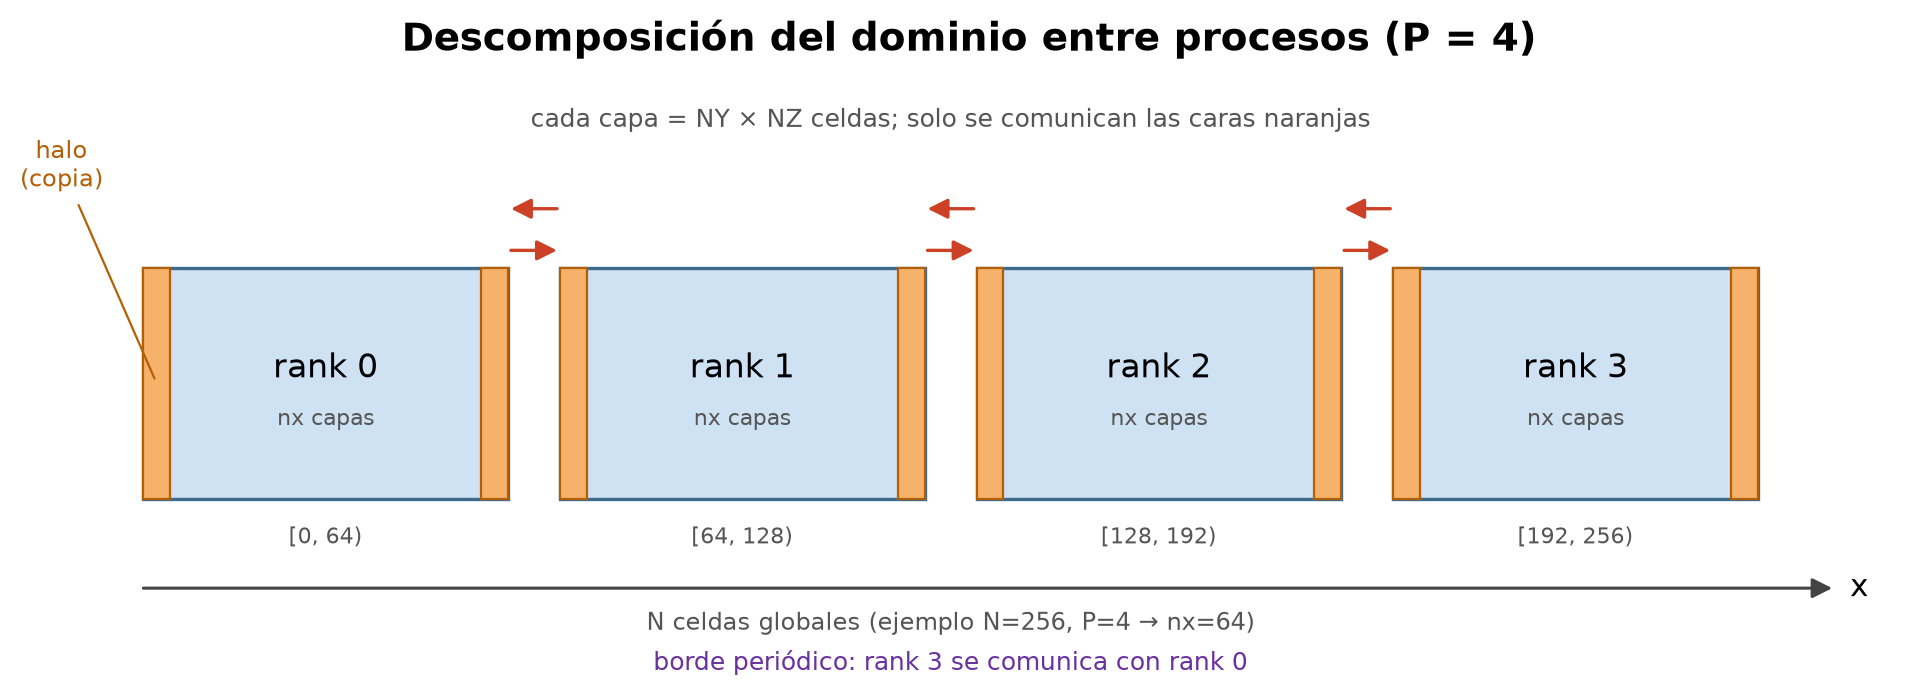
\includegraphics[width=\textwidth]{decomposition.png}
\caption{Descomposición 1D en $x$ para $P=4$: cada rank recibe $n_x$ capas y
dos capas fantasma. Solo las caras naranjas se comunican; los bordes $y,z$ son
copias locales.}
\label{fig:domain}
\end{figure}

\begin{figure}[H]
\centering
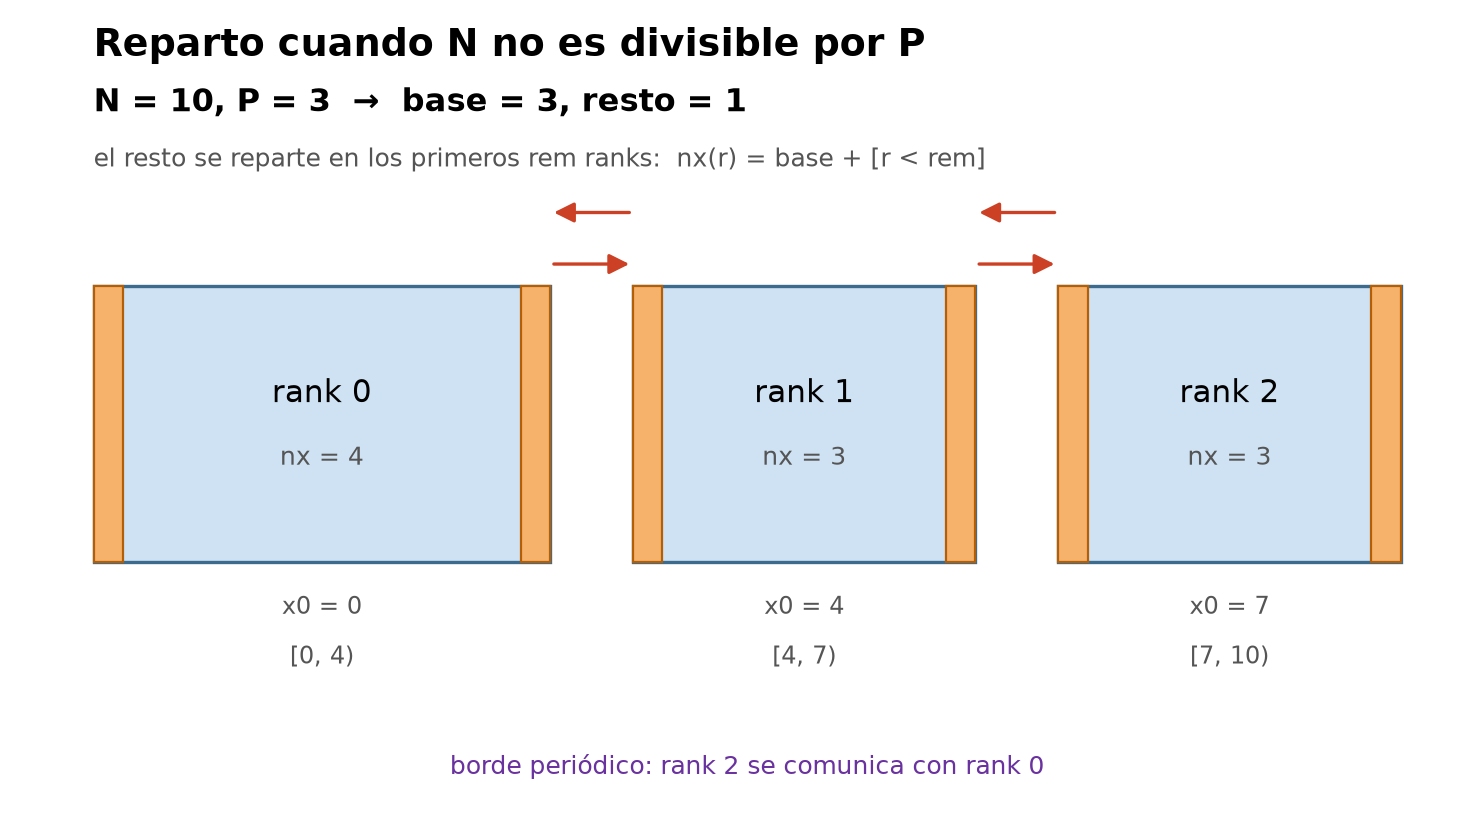
\includegraphics[width=0.92\textwidth]{decomposition_uneven.png}
\caption{Ejemplo con $N=10$, $P=3$: el resto se reparte en los primeros
$N\bmod P$ ranks. El rank 0 recibe 4 capas y los ranks 1 y 2 reciben 3.}
\label{fig:uneven}
\end{figure}

\begin{table}[H]
\centering
\caption{Reparto concreto para $N=10$, $P=3$. Los vecinos son periódicos.}
\label{tab:uneven}
\begin{tabular}{rrrcrr}
\toprule
rank & $n_x$ & $x_0$ & rango & vecino izq. & vecino der. \\
\midrule
0 & 4 & 0 & $[0,4)$ & 2 & 1 \\
1 & 3 & 4 & $[4,7)$ & 0 & 2 \\
2 & 3 & 7 & $[7,10)$ & 1 & 0 \\
\bottomrule
\end{tabular}
\end{table}

\subsection{Intercambio de halos}

Cada rank registra dos buffers, \texttt{ghost\_lo} y \texttt{ghost\_hi}, con
\texttt{bsp\_push\_reg}. En cada paso:
\begin{lstlisting}[style=cpp]
bsp_put(left,  &tmp[idx(0, -1, -1)],    ghost_hi.data(), 0, bytes);
bsp_put(right, &tmp[idx(nx - 1, -1, -1)], ghost_lo.data(), 0, bytes);
bsp_sync();
memcpy(&tmp[idx(-1, -1, -1)], ghost_lo.data(), bytes);
memcpy(&tmp[idx(nx, -1, -1)], ghost_hi.data(), bytes);
\end{lstlisting}
El halo bajo recibe la frontera alta del vecino izquierdo y viceversa. Para
$P=1$ el anillo se cierra localmente, sin comunicación.

\begin{figure}[H]
\centering
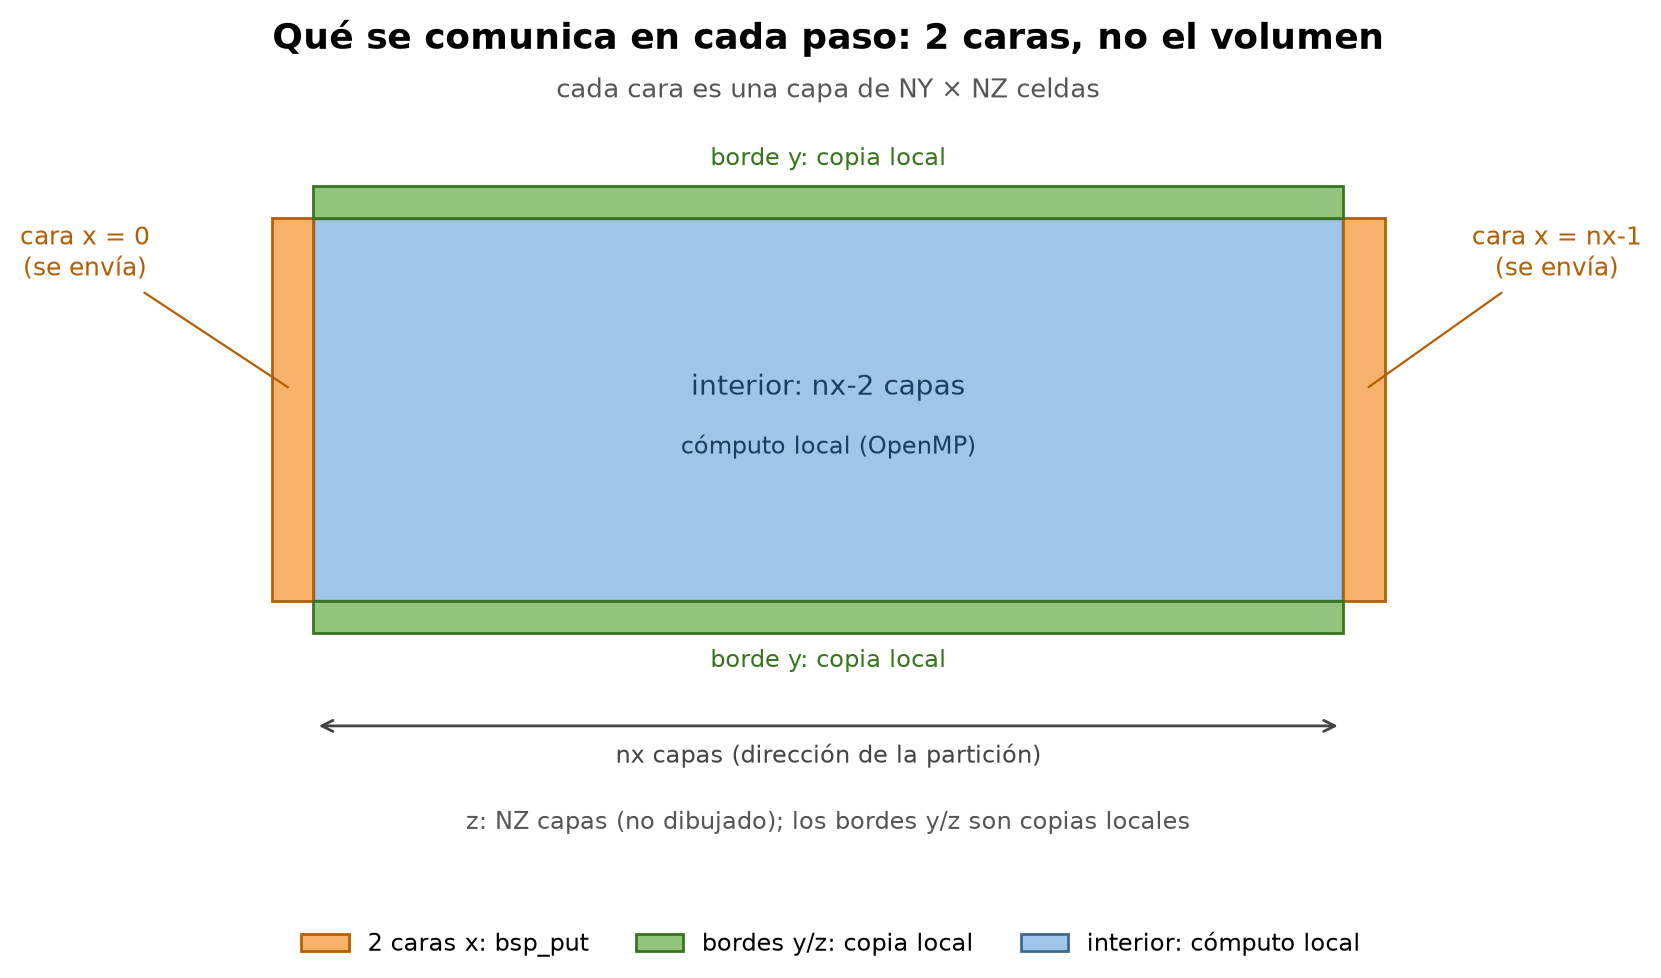
\includegraphics[width=0.90\textwidth]{communication_volume.png}
\caption{Qué se comunica en cada paso: solo las dos caras en $x$. Los bordes
$y,z$ son copias locales y el interior se calcula con OpenMP.}
\label{fig:commvolume}
\end{figure}

\begin{figure}[H]
\centering
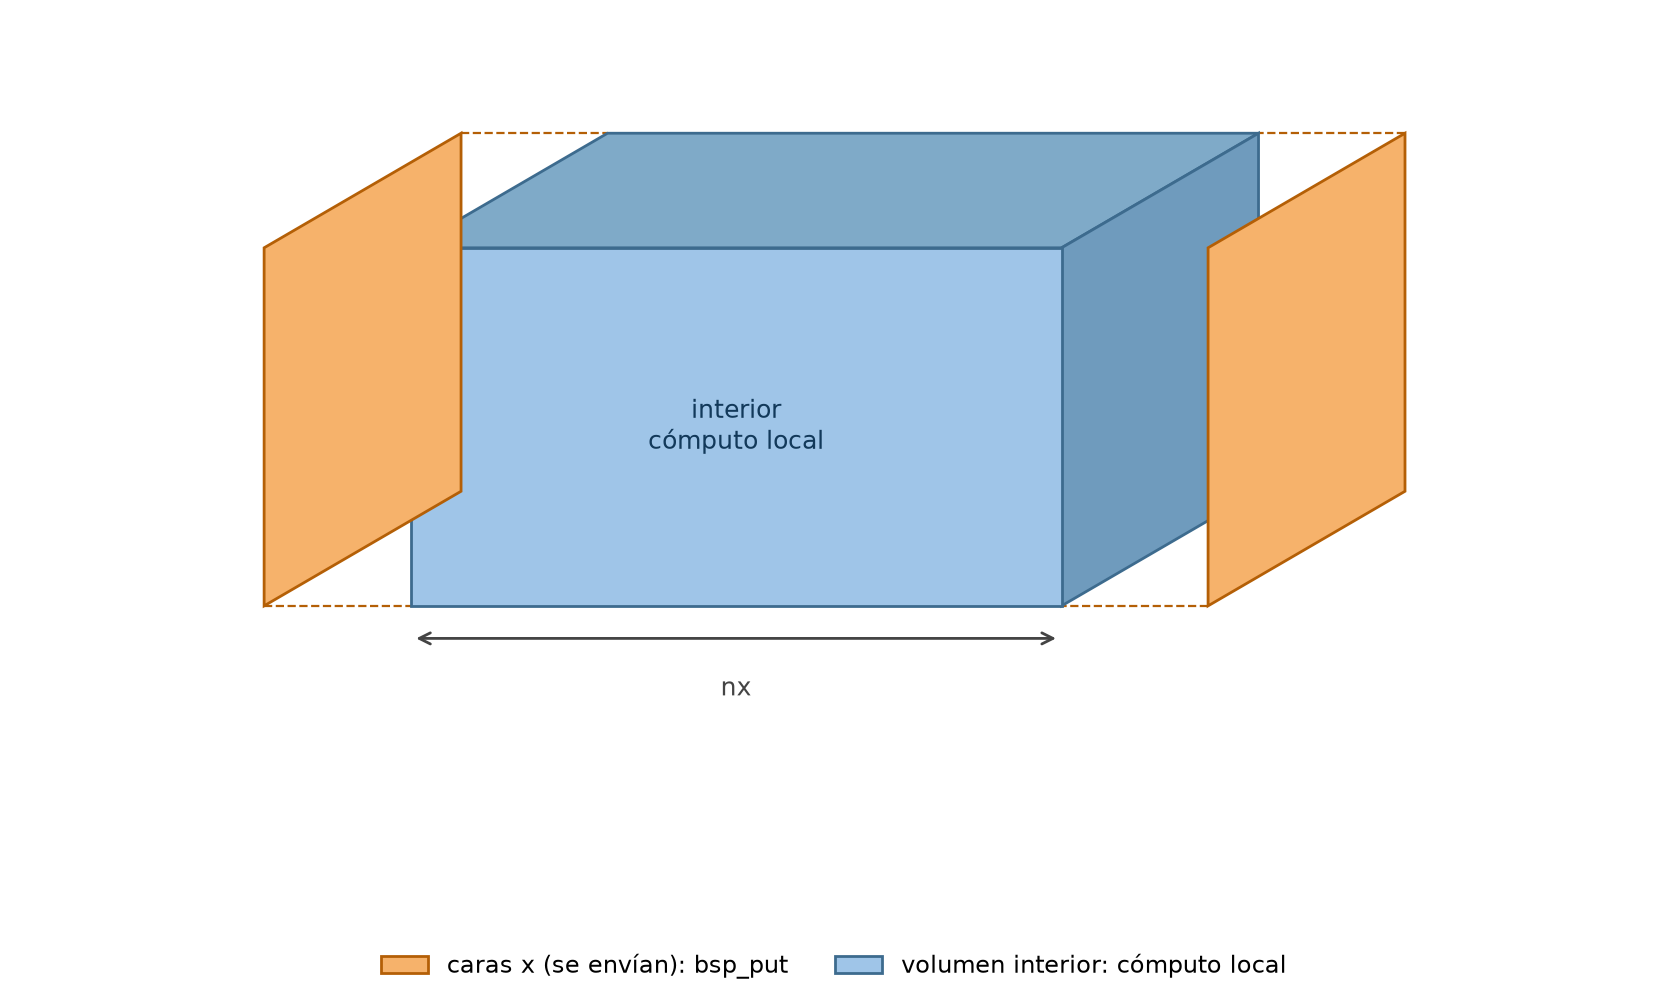
\includegraphics[width=0.78\textwidth]{communication_volume_3d.png}
\caption{Vista 3D del subdominio local: solo las dos caras en $x$ se envían;
el volumen interior se calcula localmente.}
\label{fig:comm3d}
\end{figure}

\begin{figure}[H]
\centering
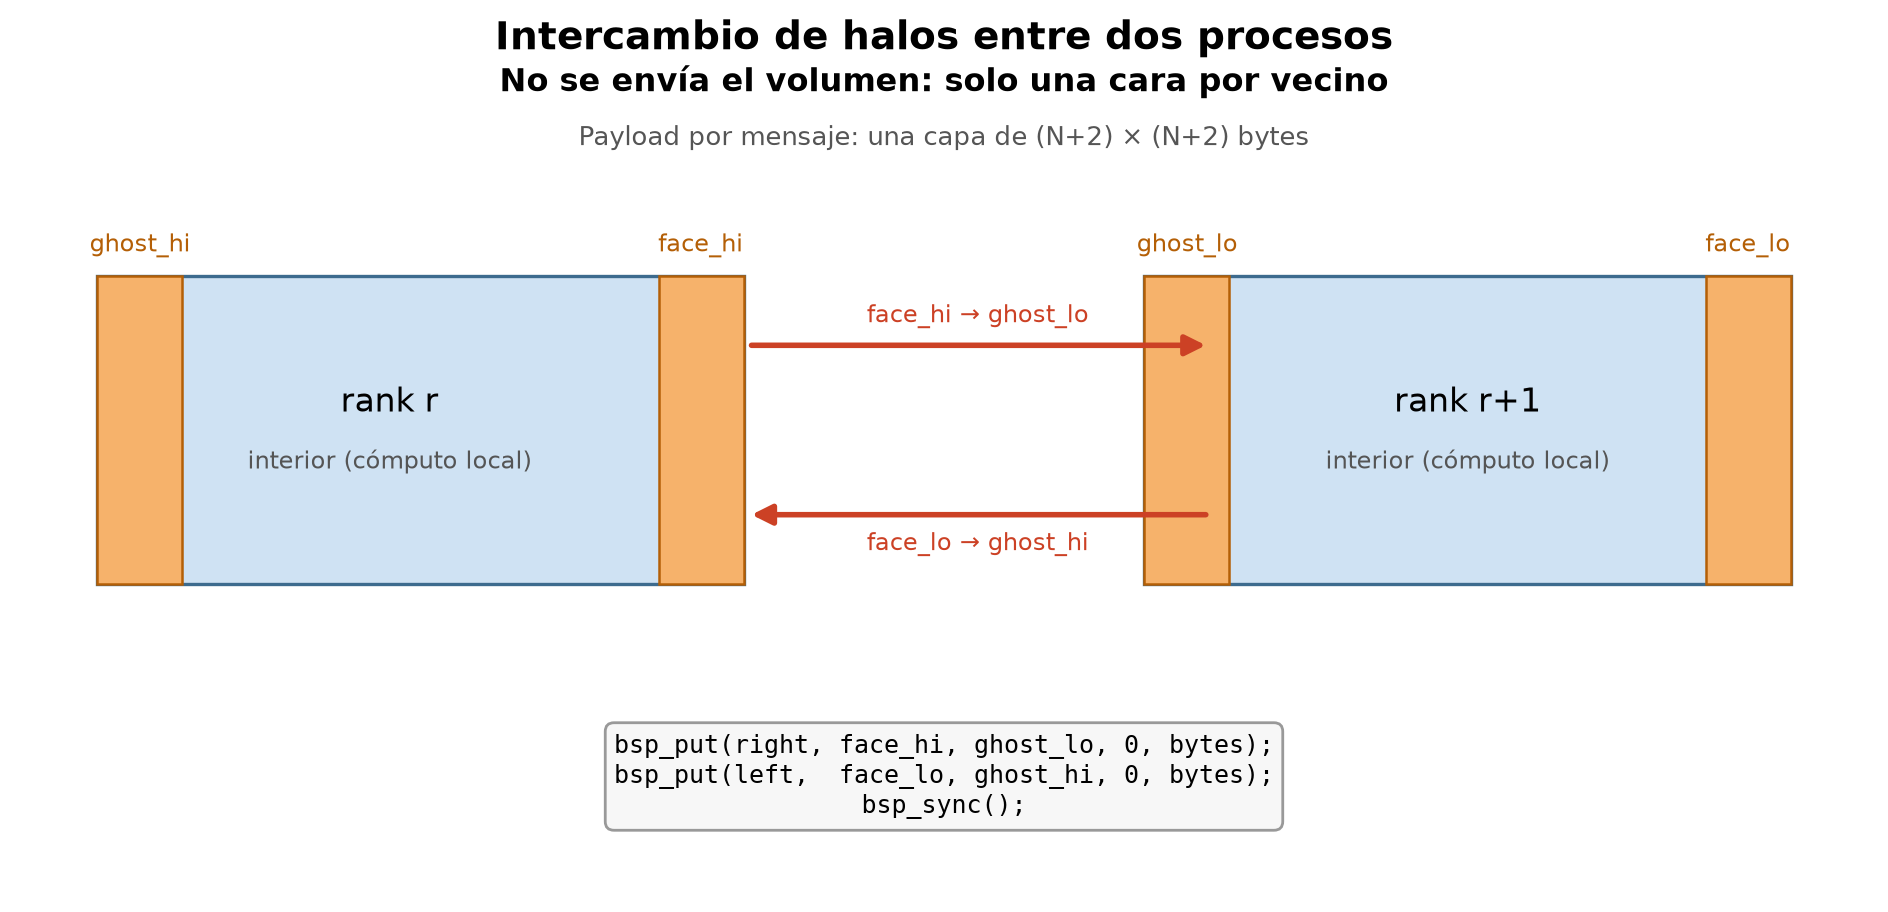
\includegraphics[width=\textwidth]{halo_exchange.png}
\caption{Detalle del intercambio: \texttt{face\_hi} se escribe en
\texttt{ghost\_lo} del vecino derecho y \texttt{face\_lo} en
\texttt{ghost\_hi} del izquierdo. La comunicación se hace visible en
\texttt{bsp\_sync}.}
\label{fig:halo}
\end{figure}

\subsection{Hilos}

OpenMP paraleliza las fases de colisión, streaming, métricas y densidad con
\texttt{\#pragma omp parallel for collapse(3)}. BSPlib no es thread-safe: todas
las llamadas van desde el hilo maestro, fuera de las regiones paralelas. El
patrón es una región OpenMP por fase, con su barrera implícita, seguida de la
comunicación serial.

\begin{figure}[H]
\centering
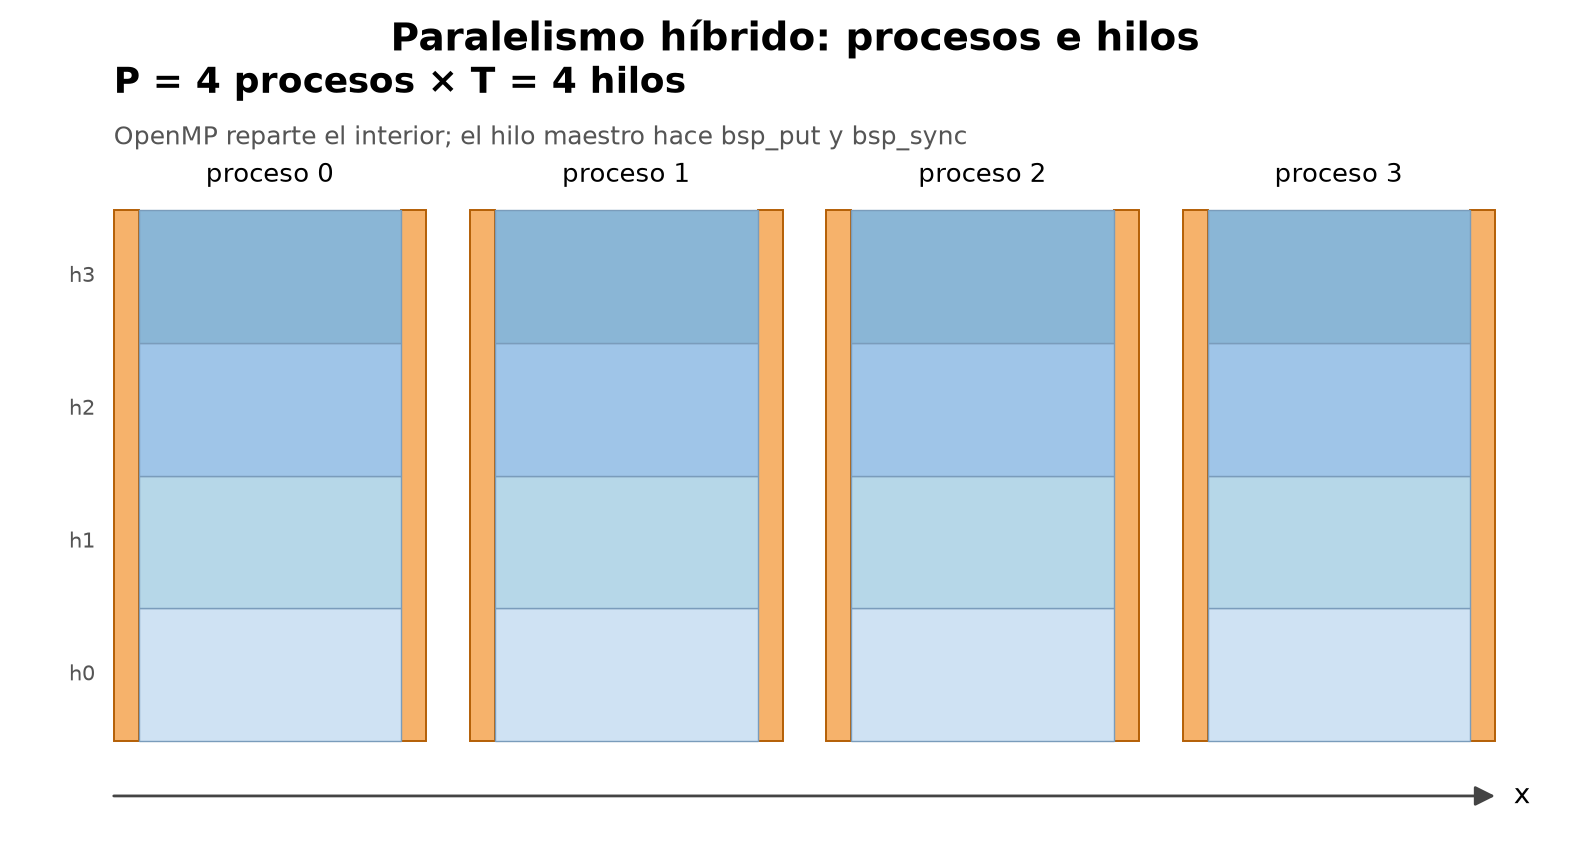
\includegraphics[width=0.82\textwidth]{hybrid_threads.png}
\caption{Paralelismo híbrido: $P=4$ procesos y $T=4$ hilos. OpenMP reparte el
interior; el hilo maestro ejecuta \texttt{bsp\_put} y \texttt{bsp\_sync}.}
\label{fig:hybrid}
\end{figure}

\subsection{Salida}

La densidad local se calcula con \texttt{popcount} y se envía a rank 0 con
\texttt{bsp\_send}. Rank 0 arma la malla global y escribe un archivo
\texttt{.vti} (XML ImageData, datos binarios \emph{appended}) que se abre en
ParaView. Las métricas globales y los tiempos se reducen de la misma forma.
El diagnóstico temporal puede volcar un CSV con el perfil $\rho(x,t)$ y
métricas por paso (variable \texttt{PROFILE\_CSV}).

\subsection{Costo BSP}

El costo de un superpaso se modela como
\begin{equation}
  T = \max_i w_i + \max_i h_i g + l,
\end{equation}
donde $w_i$ es el cómputo local, $h_i$ el volumen de comunicación, $g$ el costo
por palabra y $l$ la latencia de la barrera. En la práctica se mide la
fracción de comunicación como \texttt{comm\_max}/\texttt{time\_loop}.

Con $N=256$, cada cara mide $(N+2)^2=66.6$ KB; cada rank envía dos caras, es
decir $133$ KB por paso. Con $P=4$, el total es $0.53$ MB por paso
($0.53$ GB en 1000 pasos). El volumen local por rank es
$n_xN^2\approx4.2$ MB, así que la comunicación representa cerca del $3\%$ del
volumen local por paso; el costo dominante es la latencia de la barrera y el
alltoall de BSPonMPI, no el ancho de banda.

% ---------------------------------------------------------------------------
\section{Implementación}
% ---------------------------------------------------------------------------

\subsection{Stack y estructura}

\begin{itemize}[leftmargin=*]
  \item C++17, OpenMP, MPI (OpenMPI 4.1.6) y BSPonMPI 0.3.
  \item \texttt{src/gas.cpp}: autómata, driver BSP/OpenMP, VTK y diagnóstico.
  \item \texttt{tests/hello.cpp} y \texttt{tests/halo.cpp}: tests de humo.
  \item \texttt{docker/Dockerfile}: entorno reproducible.
  \item \texttt{scripts/}: build, run, scaling y figuras.
  \item \texttt{docs/JUSTIFICACION\_GAS\_IDEAL.md}: justificación física.
\end{itemize}

\subsection{Compilación y ejecución}

\begin{lstlisting}[language=bash,style=cpp]
docker build -t hpc-lab2:latest -f docker/Dockerfile .
./scripts/docker_shell.sh bash -lc './scripts/build.sh'
OMP_NUM_THREADS=4 mpirun -np 4 --bind-to none \
    ./build/gas 256 1000 4 0 gas
\end{lstlisting}

Con OpenMPI 4.x es obligatorio compilar con \texttt{-DOMPI\_SKIP\_MPICXX}
(el \texttt{CMakeLists.txt} ya lo define). La opción \texttt{--bind-to none}
evita que OpenMPI ate cada rank a un núcleo y ahogue a los hilos.

\subsection{Interfaz}

\begin{lstlisting}[language=bash,style=cpp]
GEOM=chamber P_RATIO=10 RAMP=8 \
GAS=neon DX_MM=1 T0_K=300 P0_ATM=1 \
OMP_NUM_THREADS=4 mpirun -np 4 --bind-to none \
    ./build/gas 256 1000 4 100 chamber
\end{lstlisting}

Las variables principales son \texttt{N}, \texttt{pasos}, \texttt{hilos},
\texttt{cada\_cuanto\_vtk} y \texttt{prefijo} (posicionales), y
\texttt{GAS}, \texttt{DX\_MM}, \texttt{T0\_K}, \texttt{P0\_ATM},
\texttt{GEOM}, \texttt{RHO\_H}, \texttt{RHO\_L}, \texttt{P\_RATIO},
\texttt{IFACE\_FRAC}, \texttt{RAMP}, \texttt{PROFILE\_CSV},
\texttt{PROFILE\_EVERY} (entorno).

% ---------------------------------------------------------------------------
\section{Validación}
% ---------------------------------------------------------------------------

\subsection{Conservación de invariantes}

\begin{table}[H]
\centering
\caption{Masa y momento antes/después en distintas configuraciones.}
\label{tab:valid}
\begin{tabular}{lrrrr}
\toprule
Caso & $P$ & $N$ & masa & momento \\
\midrule
Esfera & 1, 2, 3, 4 & 64, 256 & constante & constante \\
Esfera, $N$ impar & 2 & 63 & constante & constante \\
Cámara 10:1 & 1, 2, 4 & 64, 256 & constante & constante \\
\bottomrule
\end{tabular}
\end{table}

Los valores observados para la esfera son $M=6589$ ($N=64$) y $M=412365$
($N=256$); para la cámara $10{:}1$ con $N=256$, $M=16357802$. En todos los
casos la masa final es idéntica a la inicial y el momento se conserva.

\subsection{Comparación serial vs.\ paralelo}

Para la misma malla y cantidad de pasos, los archivos \texttt{.vti} de $P=1$ y
$P=4$ son \textbf{idénticos byte a byte}, tanto en la esfera como en la cámara.
Esto confirma que la descomposición, los halos y el \emph{gather} de salida no
alteran la física. La comparación se hace con \texttt{cmp}.

\subsection{Salida VTK}

El prefijo de longitud del bloque binario es $N^3$, la suma de los bytes de
densidad coincide con la masa global y el XML parsea correctamente. La
figura~\ref{fig:slices} muestra cortes de la cámara en cuatro tiempos.

\begin{figure}[H]
\centering
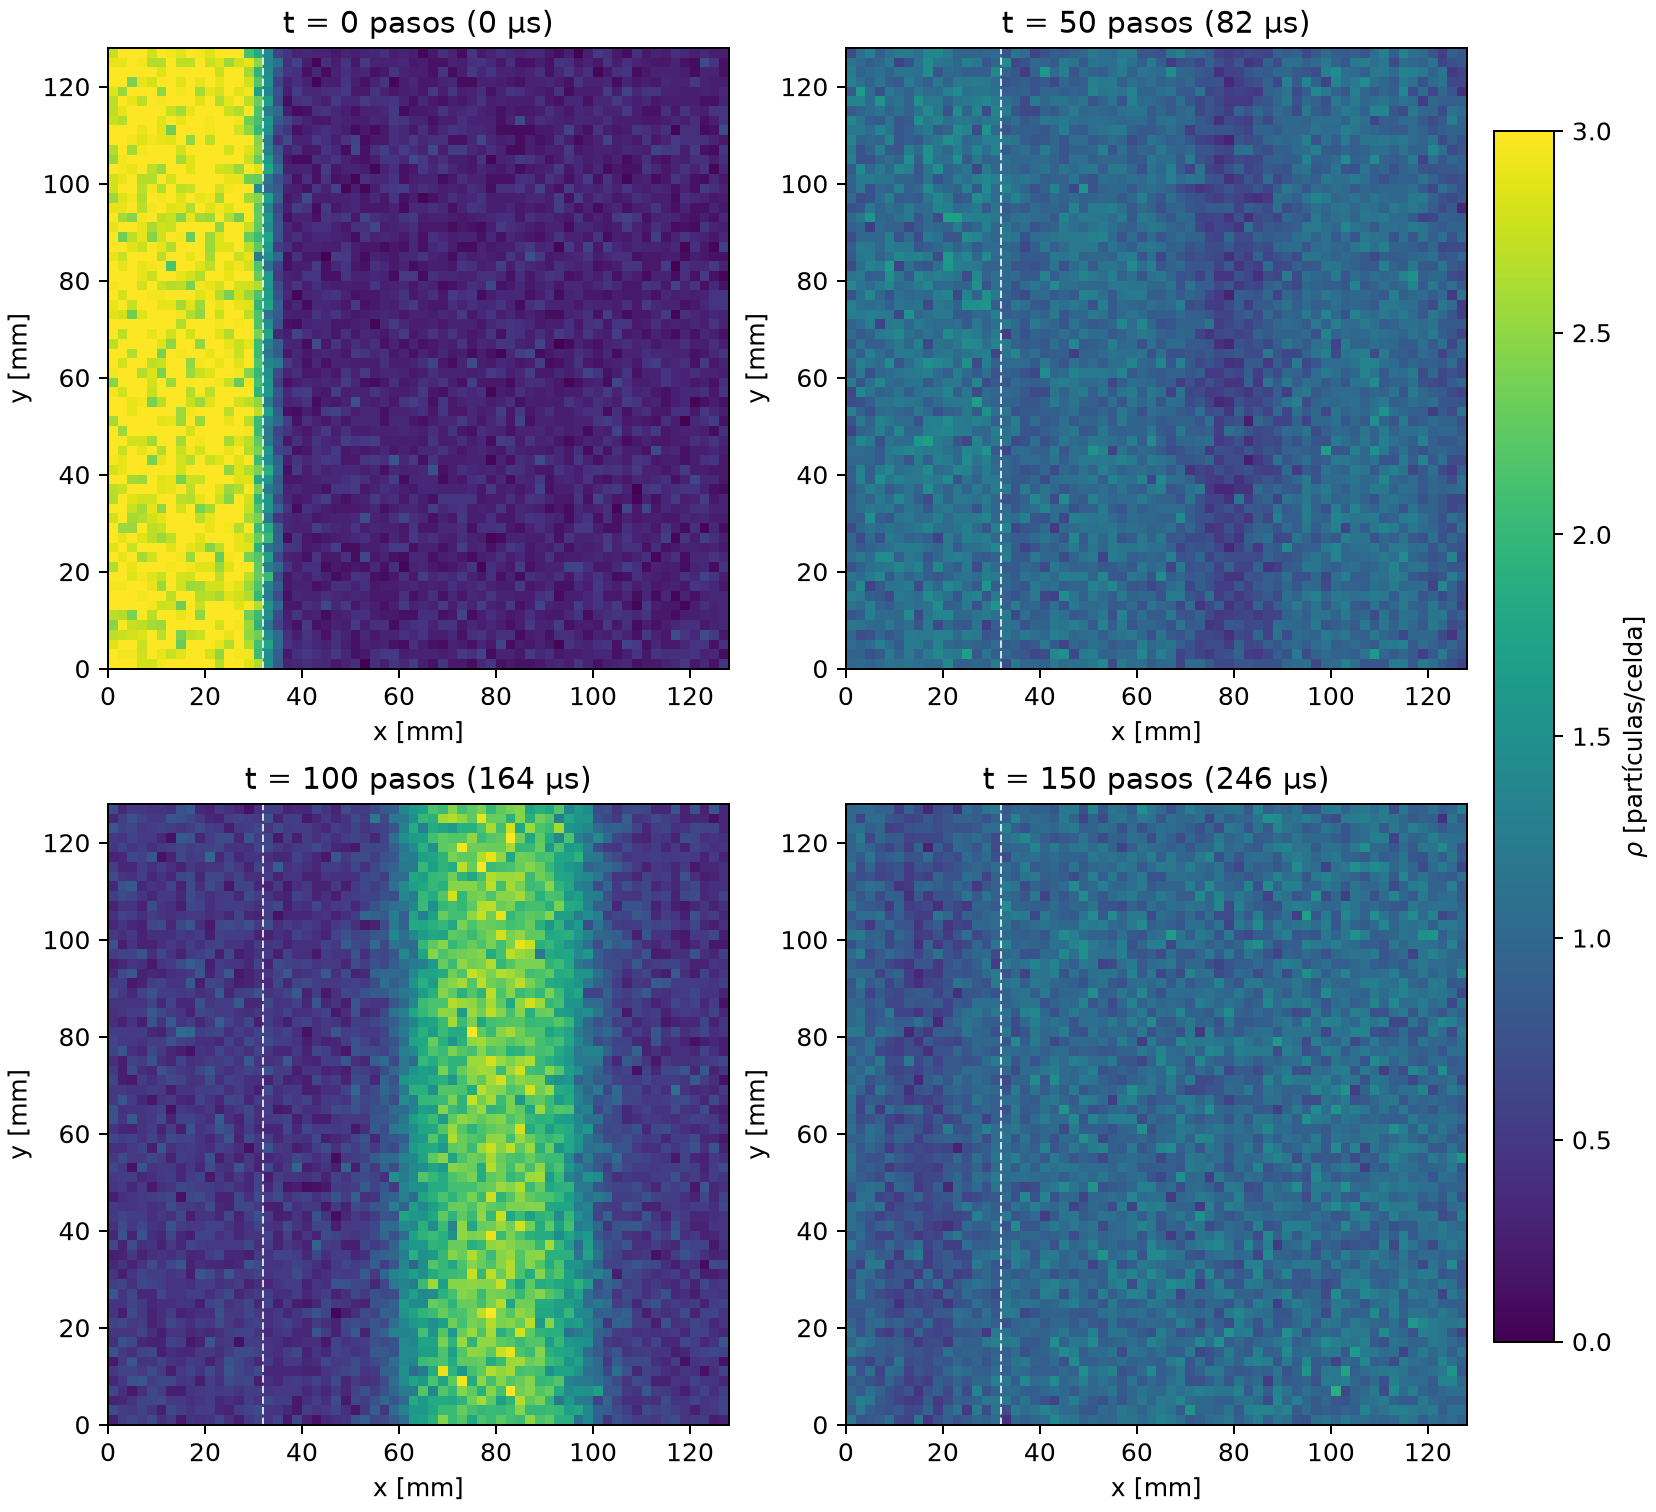
\includegraphics[width=\textwidth]{chamber_slices.png}
\caption{Cortes $z=N/2$ de la cámara $10{:}1$ con \texttt{RAMP=8}. La línea
punteada marca la interfaz inicial. Se observa la rarefacción hacia la izquierda
y la compresión hacia la derecha.}
\label{fig:slices}
\end{figure}

% ---------------------------------------------------------------------------
\section{Resultados}
% ---------------------------------------------------------------------------

\subsection{Rendimiento}

La tabla~\ref{tab:perf} resume el tiempo del loop para $N=256$ y $200$ pasos en
una laptop AMD Ryzen 7 PRO 4750U (8 núcleos, 16 hilos), dentro de Docker.

\begin{table}[H]
\centering
\caption{Tiempo del loop y speedup relativo a $1\times1$.}
\label{tab:perf}
\begin{tabular}{rrrrr}
\toprule
$P$ & $T$ & hilos totales & tiempo (s) & speedup \\
\midrule
1 & 1  & 1  & 21.27 & 1.00 \\
1 & 2  & 2  & 11.11 & 1.91 \\
1 & 4  & 4  & 6.19  & 3.44 \\
1 & 8  & 8  & 3.72  & 5.72 \\
1 & 16 & 16 & 4.04  & 5.26 \\
2 & 4  & 8  & 6.40  & 3.32 \\
4 & 2  & 8  & 6.76  & 3.15 \\
4 & 4  & 16 & 4.06  & 5.24 \\
8 & 2  & 16 & 4.18  & 5.09 \\
\bottomrule
\end{tabular}
\end{table}

\begin{figure}[H]
\centering
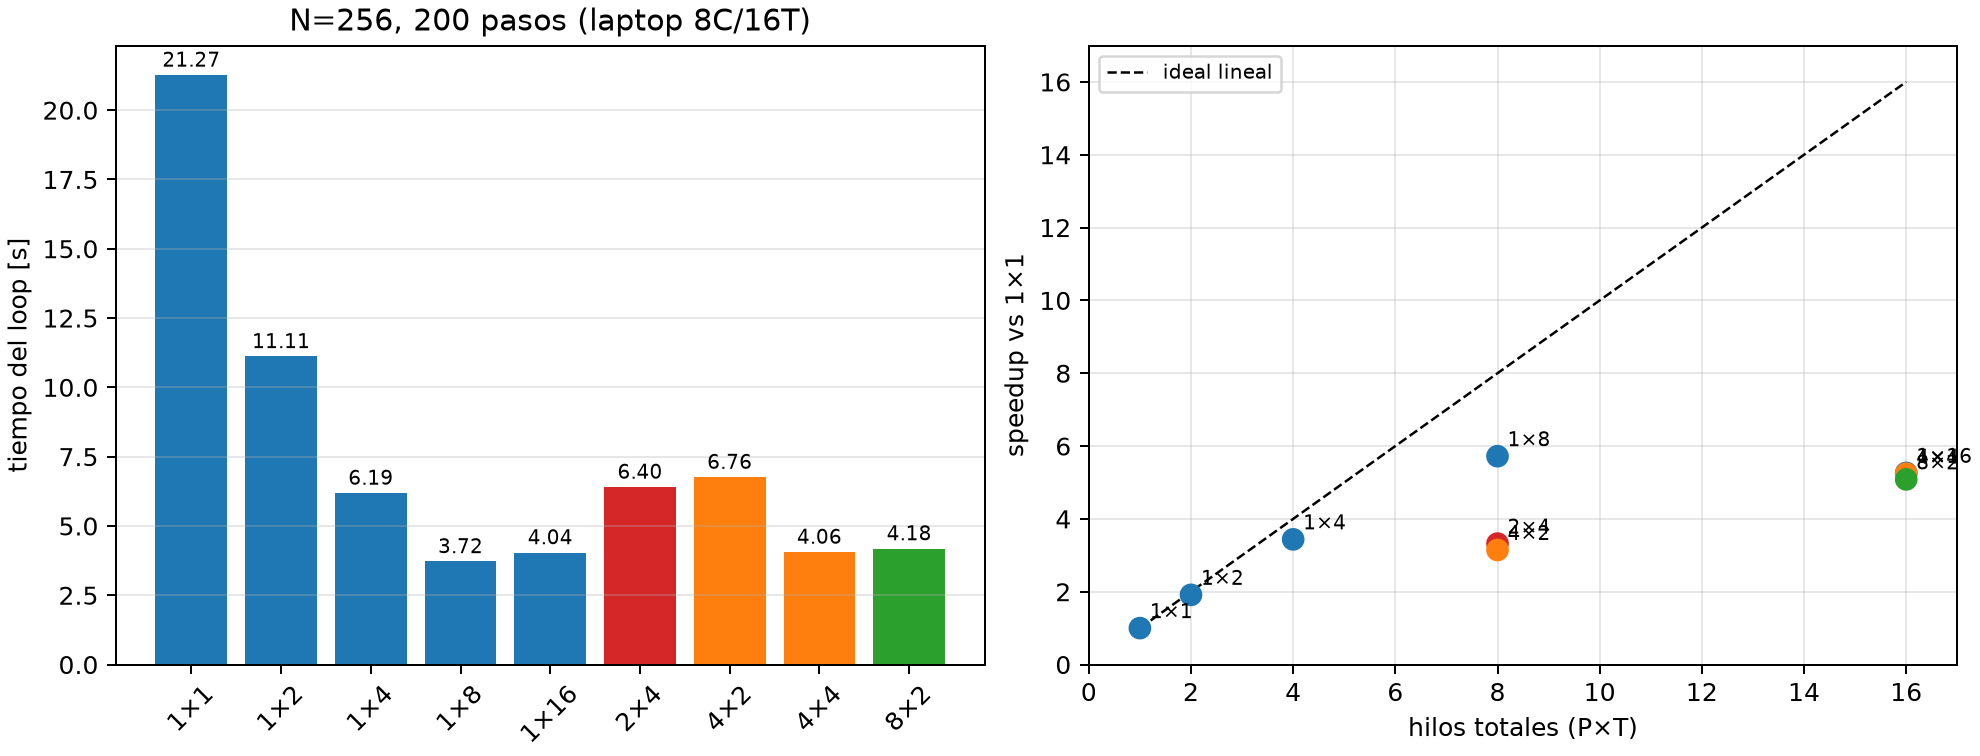
\includegraphics[width=\textwidth]{scaling.png}
\caption{Tiempo y speedup. El problema es \emph{memory-bound}: en un solo nodo
el mejor resultado es OpenMP puro ($1\times8$); los procesos agregan el costo
de la barrera BSP.}
\label{fig:scaling}
\end{figure}

\begin{figure}[H]
\centering
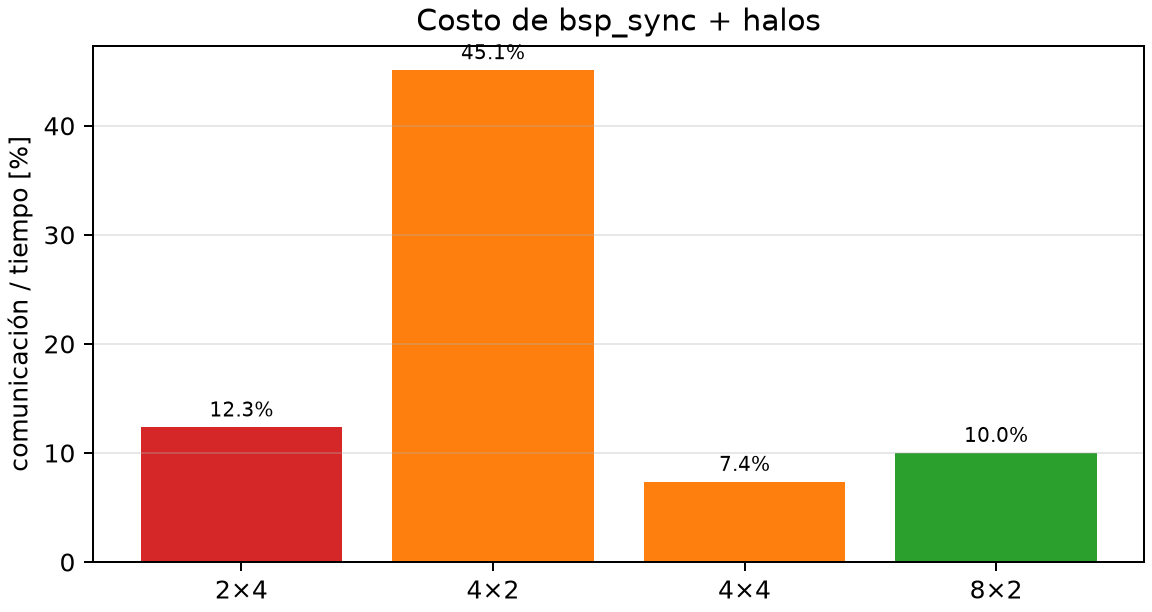
\includegraphics[width=0.62\textwidth]{comm_fraction.png}
\caption{Fracción del tiempo de loop atribuida a comunicación (halos +
\texttt{bsp\_sync}) en las configuraciones con $P>1$.}
\label{fig:comm}
\end{figure}

\subsection{Evolución temporal}

El diagnóstico \texttt{PROFILE\_CSV} vuelca el perfil $\rho(x,t)$ y métricas
globales por paso. La figura~\ref{fig:spacetime} muestra el diagrama
espacio-temporal de la cámara: se ven la onda de rarefacción (izquierda), la
interfaz y la compresión que viaja a la derecha. La
figura~\ref{fig:metrics} resume densidad máxima del perfil, centro de masa,
ancho RMS y fracción de masa que cruzó la interfaz. La animación de la
evolución está en \texttt{docs/figs/evolution\_chamber.gif}.

\begin{figure}[H]
\centering
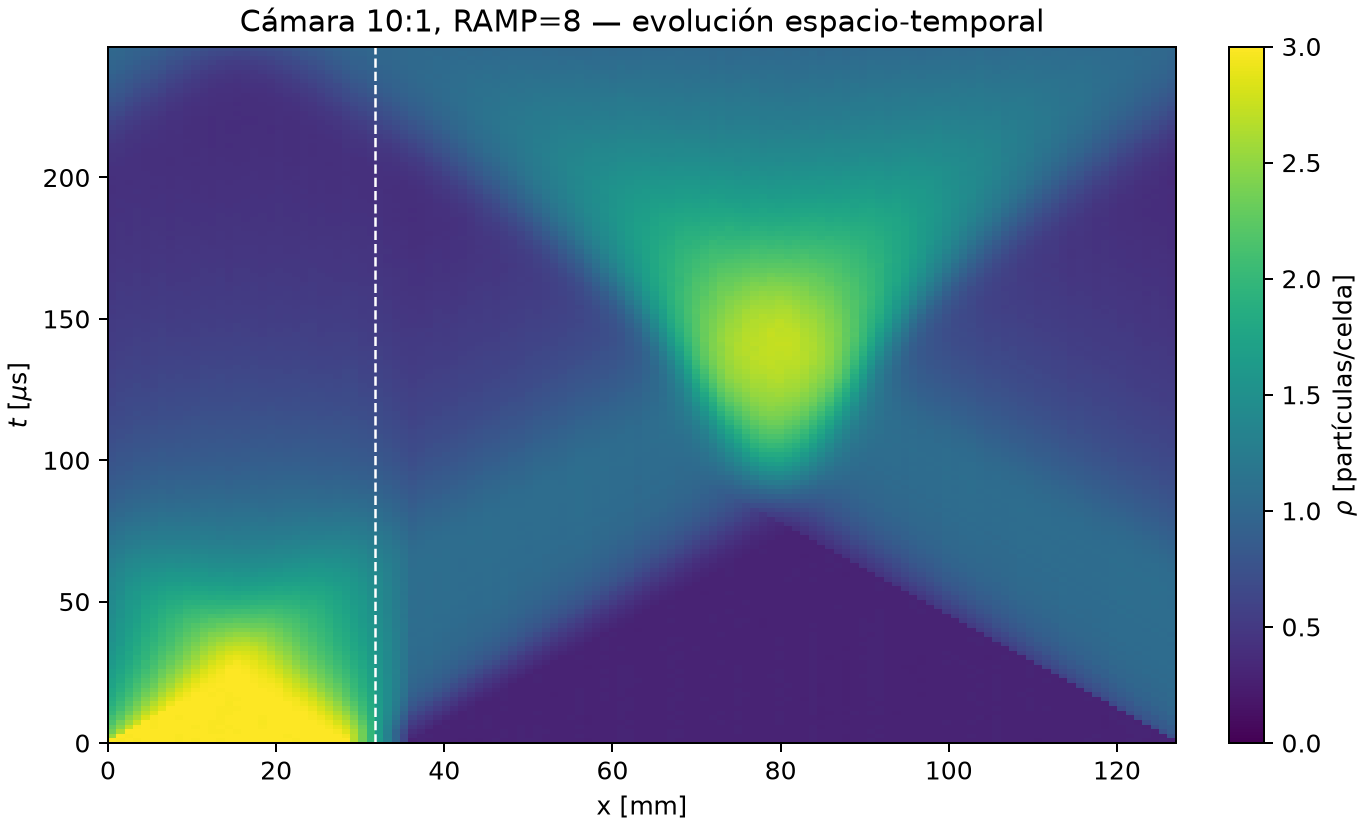
\includegraphics[width=0.88\textwidth]{spacetime_chamber.png}
\caption{Diagrama espacio-temporal de la cámara $10{:}1$ con \texttt{RAMP=8}.
El eje vertical es tiempo físico ($\mu$s) y el color es la densidad media en
$x$. La línea punteada es la interfaz inicial.}
\label{fig:spacetime}
\end{figure}

\begin{figure}[H]
\centering
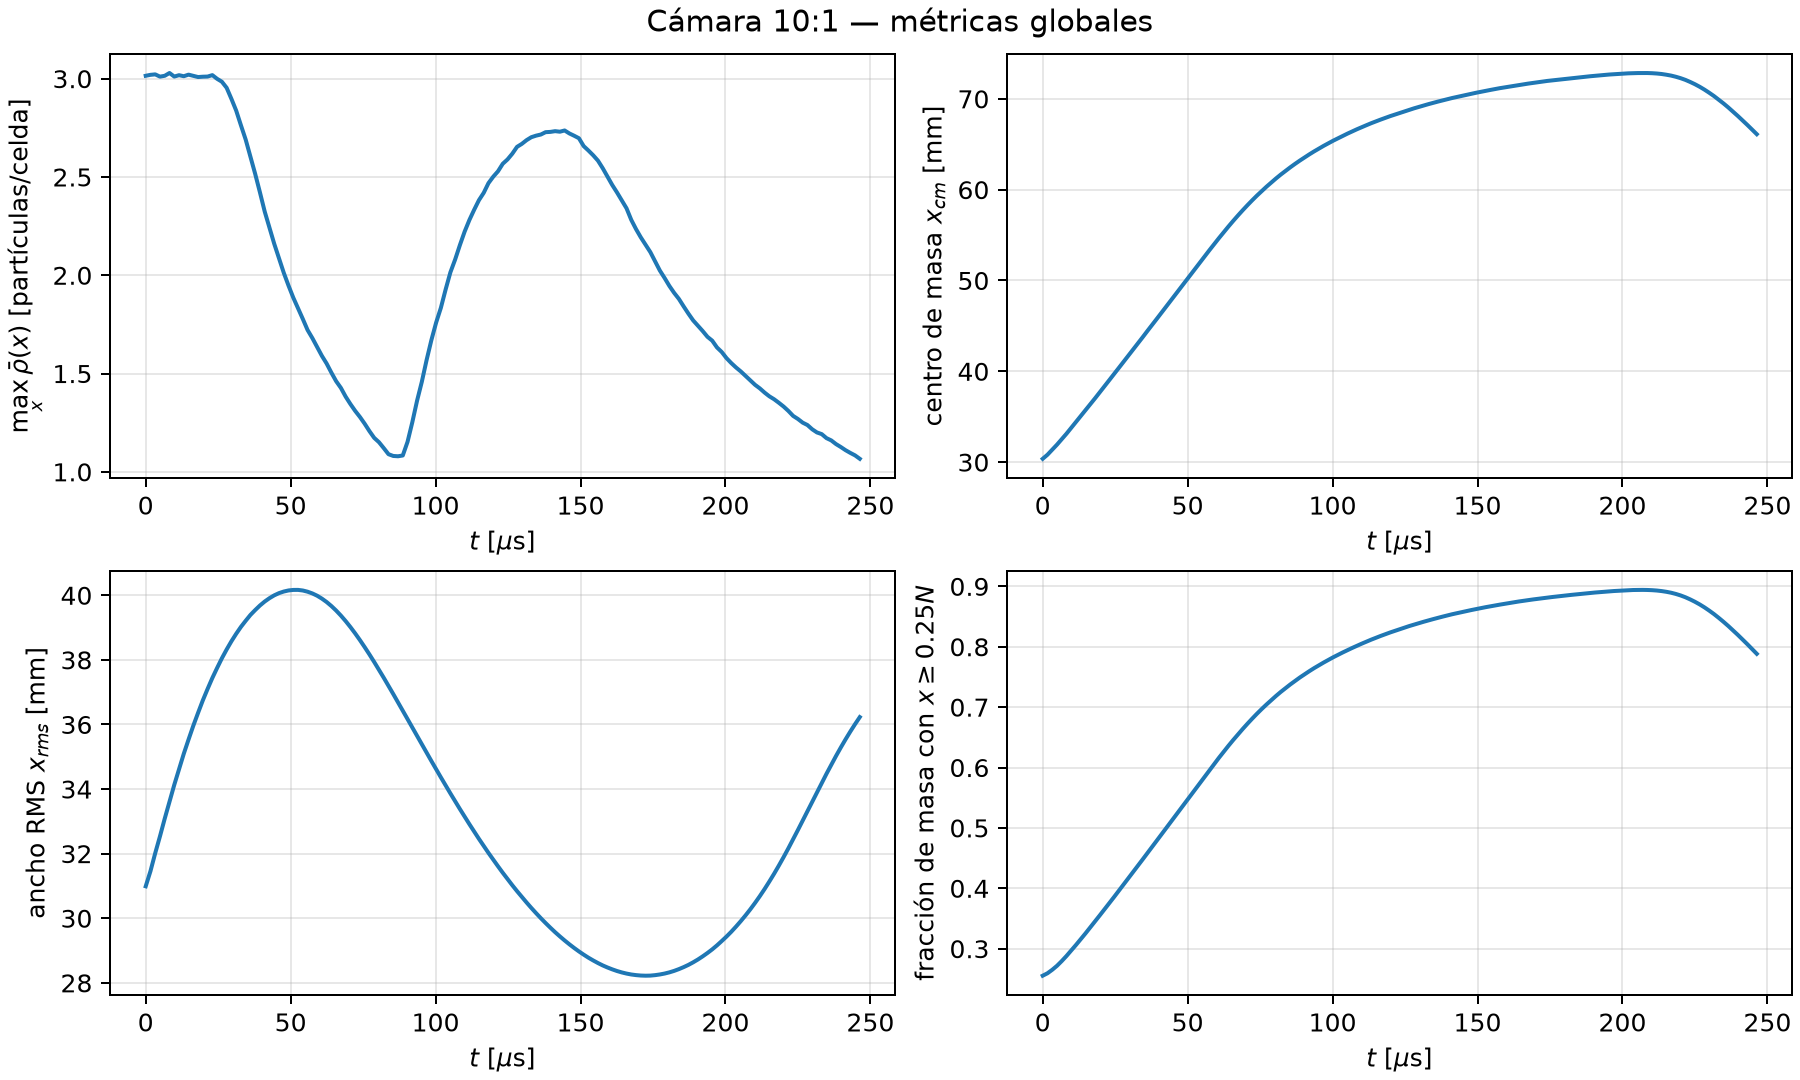
\includegraphics[width=\textwidth]{evolution_chamber.png}
\caption{Métricas globales de la cámara: máximo del perfil, centro de masa,
ancho RMS y fracción de masa con $x\ge 0.25N$.}
\label{fig:metrics}
\end{figure}

\subsection{Discusión}

\begin{itemize}[leftmargin=*]
  \item El problema es \emph{memory-bound}: el streaming y la tabla de colisión
        dominan; agregar hilos ayuda hasta saturar los 8 núcleos físicos.
  \item En un solo nodo, OpenMP puro ($1\times8$) es apenas mejor que
        $4\times4$; la capa de procesos no reduce el tiempo porque el
        \texttt{bsp\_sync}/alltoall de BSPonMPI compensa la división del
        trabajo.
  \item La fracción de comunicación es baja en $4\times4$ ($\approx7\%$) pero
        alta en $4\times2$ ($\approx45\%$), donde hay poco trabajo por rank.
  \item El objetivo $4\times8$ requiere un nodo de 32 hilos; en esta laptop
        $4\times4$ es la configuración híbrida razonable.
  \item La comparación byte a byte serial/paralelo es una validación fuerte de
        la corrección del esquema híbrido.
\end{itemize}

% ---------------------------------------------------------------------------
\section{Conclusiones y trabajo futuro}
% ---------------------------------------------------------------------------

Se implementó y validó un autómata celular 3D para la expansión de un gas con
paralelismo híbrido BSPlib + OpenMP. La masa y el momento se conservan
exactamente, la salida paralela coincide byte a byte con la serial y el esquema
de halos funciona para $P$ arbitrario, incluso si $P$ no divide a $N$. El mapeo
a neón permite reportar magnitudes físicas reales y la cámara de dos presiones
da un gradiente explícito.

Trabajo futuro:
\begin{enumerate}[leftmargin=*]
  \item Correr $4\times8$ en un nodo de 32 hilos y completar weak scaling.
  \item Agregar paredes reflectantes para un recipiente cerrado.
  \item Evaluar un LGA térmico (partícula en reposo, energía) para expansión
        adiabática.
  \item Exportar presión/velocidad al VTK y generar animaciones 3D.
  \item Optimizar el streaming (eliminar ramas, \texttt{-march=native},
        vectorización) y explorar descomposición 2D/3D.
\end{enumerate}

% ---------------------------------------------------------------------------
\begin{thebibliography}{9}

\bibitem{valiant}
L.~G. Valiant, \emph{A Bridging Model for Parallel Computation},
Communications of the ACM, 33(8):103--111, 1990.

\bibitem{bsplib}
J.~M.~D. Hill, B.~McColl, D.~C. Stefanescu, M.~W. Goudreau, K.~Lang,
S.~B. Rao, T.~Suel, T.~Tsantilas y R.~Bisseling,
\emph{BSPlib: The BSP Programming Library}, Parallel Computing, 24:1947--1980,
1998.

\bibitem{bsponmpi}
W.~J. Suijlen, \emph{BSPonMPI: BSPlib on top of MPI},
\url{https://sourceforge.net/projects/bsponmpi/}.

\bibitem{fhp}
U.~Frisch, B.~Hasslacher y Y.~Pomeau,
\emph{Lattice-Gas Automata for the Navier--Stokes Equation},
Physical Review Letters, 56:1505, 1986.

\bibitem{virial}
J.~H. Dymond y E.~B. Smith,
\emph{The Virial Coefficients of Pure Gases and Mixtures},
Oxford University Press, 1980.

\bibitem{openmp}
OpenMP Architecture Review Board, \emph{OpenMP Application Programming
Interface}, \url{https://www.openmp.org/}.

\end{thebibliography}

% ---------------------------------------------------------------------------
\appendix
\section{Detalles de BSPonMPI}

BSPonMPI implementa BSPlib sobre MPI. Puntos a tener en cuenta:
\begin{itemize}[leftmargin=*]
  \item \texttt{bsp\_init} es obligatorio.
  \item \texttt{bsp\_get\_tag} devuelve el tamaño del payload \emph{más} el
        tag; hay que restar \texttt{sizeof(int)} antes de \texttt{bsp\_move}.
  \item Varias funciones usan \texttt{size\_t} en lugar de \texttt{int}:\\
        \texttt{bsp\_push\_reg}, \texttt{bsp\_qsize}, \texttt{bsp\_move},
        \texttt{bsp\_set\_tagsize}.
  \item No implementa las colectivas \texttt{bsp\_bcast}/\allowbreak
        \texttt{bsp\_fold} ni las funciones de costo
        \texttt{bsp\_l}/\allowbreak \texttt{bsp\_s}/\allowbreak
        \texttt{bsp\_g}.
  \item \texttt{bsp\_put} y \texttt{bsp\_send} son diferidos hasta
        \texttt{bsp\_sync}.
\end{itemize}

\section{Reproducibilidad}

\begin{lstlisting}[language=bash,style=cpp]
# entorno
docker build -t hpc-lab2:latest -f docker/Dockerfile .
./scripts/docker_shell.sh bash -lc './scripts/build.sh'

# tests
./scripts/docker_shell.sh bash -lc 'mpirun -np 4 --bind-to none ./build/hello 4'
./scripts/docker_shell.sh bash -lc 'mpirun -np 4 --bind-to none ./build/halo_test 4'

# scaling
N=256 STEPS=200 P_VALUES="1 2 4 8" T_VALUES="1 2 4 8" \
  ./scripts/docker_shell.sh bash -lc './scripts/scaling.sh'

# figuras (requiere los .vti y los CSV en data/figs)
python3 scripts/make_figures.py
python3 scripts/plot_evolution.py
\end{lstlisting}

\end{document}
